\section{Resultados}
\subsection{Poblaciones reconstruidas a 50 MeV}
La entrada cosmológica central fijó $Y_{\Delta B}^{\rm ref}=8.69318\times10^{-11}$. Con ese mismo exceso por unidad de entropía, el HRG PDG2025 a 50 MeV ($5.8023\times10^{11}$ K) produjo $n_B=2.7261\times10^{30}$ y $n_{\bar B}=2.7172\times10^{30}$ cm$^{-3}$. La suma fue $5.4433\times10^{30}$ cm$^{-3}$ y el exceso neto, $8.8765\times10^{27}$ cm$^{-3}$ (Tabla~\ref{tab:states}). Estas cuatro cifras son resultados del cálculo inverso; el rendimiento neto fue la condición externa impuesta.

El cociente $R=306.1147$ significa que por cada unidad del exceso neto coexistieron aproximadamente 306.1 antibariones y 307.1 bariones en ese estado. Se obtuvo $n_{\bar B}/n_B=0.996744$: unos 99.6744 antibariones por cada 100 bariones. El exceso representó 0.163071\% de la suma. La solución requirió $\mu_B/T=0.00163071$, equivalente a $\mu_B=0.0815356$ MeV.

\begin{table*}[t]\centering\small
\caption{Estados reconstruidos con PDG2025 y el valor central de $\eta$. Las densidades corresponden al volumen físico a cada temperatura; $R=n_{\bar B}/\Delta n_B$.}
\label{tab:states}
\setlength{\tabcolsep}{6pt}
\begin{tabular}{rrrrrr}\toprule
$T$ (MeV) & $n_B$ (cm$^{-3}$) & $n_{\bar B}$ (cm$^{-3}$) & $\Delta n_B$ (cm$^{-3}$) & $R$ & $\mu_B/T$\\\midrule
50.0 & $2.7261\times10^{30}$ & $2.7172\times10^{30}$ & $8.8765\times10^{27}$ & 306.114688 & 0.001631\\
45.0 & $2.8323\times10^{29}$ & $2.7694\times10^{29}$ & $6.2899\times10^{27}$ & 44.028849 & 0.011229\\
40.0 & $1.9166\times10^{28}$ & $1.4894\times10^{28}$ & $4.2724\times10^{27}$ & 3.486095 & 0.126100\\
38.203739 & $7.3454\times10^{27}$ & $3.6727\times10^{27}$ & $3.6727\times10^{27}$ & 1.000000 & 0.346574\\
37.0 & $4.4167\times10^{27}$ & $1.1116\times10^{27}$ & $3.3051\times10^{27}$ & 0.336326 & 0.689799\\
\bottomrule\end{tabular}
\end{table*}


Los protones, neutrones y sus antipartículas aportaron 95.2176\% de la población bariónica total a 50 MeV; los demás bariones del catálogo aportaron 4.7824\%. La Tabla~\ref{tab:nucleons50} identifica las contribuciones nucleónicas con sus masas de reposo conservadas. La fracción de entropía del sector barión-antibarión fue $s_{B+\bar B}/s_{\rm tot}=1.15182\times10^{-6}$; esta fracción de entropía es distinta de una fracción de número de partículas.

\begin{table}[t]\centering\small
\caption{Nucleones y sus antipartículas a 50 MeV, PDG2025. La densidad se expresa en unidades de $10^{30}$ cm$^{-3}$.}
\label{tab:nucleons50}
\begin{tabular}{lrr}\toprule
Especie de partícula & Masa (MeV) & Densidad\\\midrule
$p$ & 938.272 & 1.313384\\
$\bar p$ & 938.272 & 1.309107\\
$n$ & 939.565 & 1.282334\\
$\bar n$ & 939.565 & 1.278159\\
\bottomrule\end{tabular}
\end{table}


\subsection{Secuencia térmica y cruce de abundancias}
Al descender de 50 a 45 y 40 MeV, $R$ pasó de 306.1147 a 44.02885 y 3.486095. A la temperatura publicada de 38.2 MeV se obtuvo $R=0.997012$; la raíz propia fue $T_\times=38.203739$ MeV (Figura~\ref{fig:cross}). El cruce redondea a 38.2 MeV a la precisión de \citet{Yang2022}. La diferencia aritmética, $+0.003739$ MeV, no proporciona una precisión estadística del acuerdo.

En la raíz PDG2025, $n_{\bar B}=\Delta n_B=3.6727\times10^{27}$ cm$^{-3}$ y $n_B=7.3454\times10^{27}$ cm$^{-3}$. Por definición, $R=1$ implica $n_B=2n_{\bar B}$, $n_{\bar B}/n_B=1/2$ y un exceso igual a un tercio de la suma. Los antibariones seguían presentes en ese hito. La participación nucleónica alcanzó 98.8254\%.

\begin{figure*}[t]
\centering
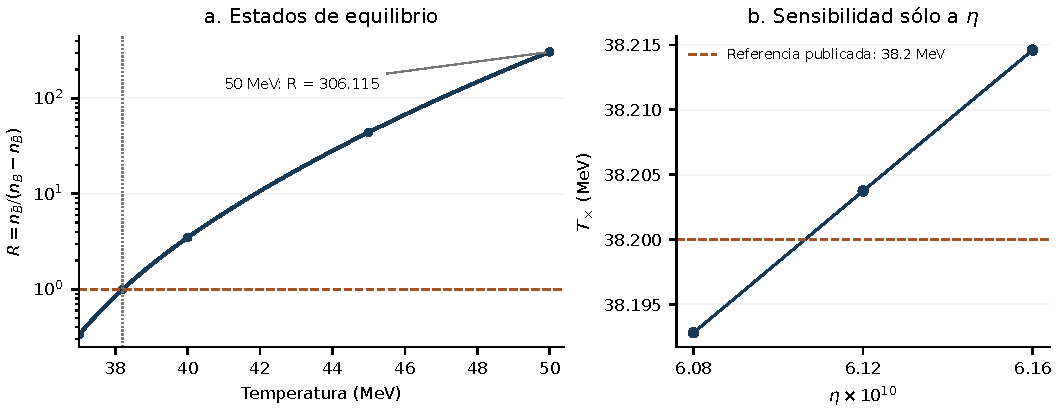
\includegraphics[width=.98\textwidth]{figures/final_cross_es.pdf}
\caption{Cociente de antibariones respecto del exceso neto para PDG2025. Izquierda: secuencia de estados de equilibrio entre 37 y 50 MeV; los puntos indican evaluaciones propias y la línea horizontal, $R=1$. Derecha: temperatura de cruce obtenida para el valor central y los extremos de la incertidumbre de entrada de $\eta$; la línea entre puntos es una guía visual. La referencia de 38.2 MeV procede de Yang y Rafelski (2022); no se le asigna una incertidumbre no publicada.}
\label{fig:cross}
\end{figure*}

Los tres inventarios dieron cruces cercanos (Tabla~\ref{tab:crosscatalogs}). Entre PDG2014 y PDG2025, la amplitud numérica fue $0.000142$ MeV. Al variar sólo $\eta$ en $(6.12\pm0.04)\times10^{-10}$, el cruce PDG2025 abarcó 38.192814--38.214598 MeV y $R(50)$ abarcó 304.1237--308.1319. Esta sensibilidad de entrada fue mayor que la diferencia con el valor bibliográfico redondeado y que la amplitud de estos tres catálogos.

\begin{table}[t]\centering\small
\caption{Sensibilidad al inventario con la misma entrada cosmológica. Los decimales adicionales documentan el cálculo, no su exactitud física.}
\label{tab:crosscatalogs}
\begin{tabular}{lrr}\toprule
Lista & $T_\times$ (MeV) & $R(50\ {\rm MeV})$\\\midrule
PDG2014 & 38.203596 & 306.128980\\
PDG2020 & 38.203739 & 306.114776\\
PDG2025 & 38.203739 & 306.114688\\
\bottomrule\end{tabular}
\end{table}


\subsection{Cantidades en una misma región comóvil}
Las conversiones cosmológicas dieron $n_{\gamma0}=410.7268$ cm$^{-3}$ y $n_{b0}=(2.514\pm0.017)\times10^{-7}$ cm$^{-3}$, compatibles con la densidad bariónica media compilada por \citet{Groom2025}. Esta compatibilidad verifica la conversión de entradas compartidas, sin constituir una predicción independiente del residuo.

La región comóvil que corresponde hoy a 1 m$^3$ contiene en promedio 0.251365 unidades de número bariónico neto. A 50 MeV, el cálculo asignó a esa misma región aproximadamente 77.1978 bariones y 76.9465 antibariones, con suma 154.1443 y la misma diferencia 0.251365. En el cruce, las cantidades fueron 0.502730 y 0.251365, respectivamente. Son cantidades medias normalizadas al volumen actual, no las densidades de un m$^3$ físico del plasma temprano ni eventos acumulados de regeneración.

La composición primordial equivalente dio $n_{H0}^{\rm prim}=(1.898\pm0.015)\times10^{-7}$, $n_{{}^4He,0}^{\rm prim}=(1.540\pm0.021)\times10^{-8}$ y $n_{D0}^{\rm prim}=(4.760\pm0.066)\times10^{-12}$ cm$^{-3}$. Estas cantidades convierten abundancias nucleares externas a la densidad media actual; el HRG de 50 MeV no predijo la producción posterior de H, He o D. La comparación común se establece a través del número bariónico neto.

\subsection{Verificación numérica e información recuperable}
Los 24 controles se completaron satisfactoriamente. La diferencia relativa máxima al pasar de 96 a 192 términos fue $4.44\times10^{-16}$ y el error relativo máximo de cierre de $Y_{\Delta B}$, $1.25\times10^{-14}$. Las integrales independientes de nucleones coincidieron con las sumas dentro de $1.23\times10^{-15}$. Estas cifras cuantifican consistencia computacional, sin medir la exactitud física del modelo.

La prueba de rango confirmó que el residuo solo aporta una ecuación para dos poblaciones: añadir el mismo rendimiento a bariones y antibariones deja intacto $Y_{\Delta B}$. El equilibrio, el inventario y la temperatura aportaron la relación adicional que permitió reconstruir las poblaciones de la Tabla~\ref{tab:states}. No se obtuvo una selección única de la historia de producción y aniquilación a partir de las abundancias presentes.
